\documentclass[11pt, titlepage]{article}
\usepackage[ugly]{thesis}
\newcommand{\norm}[1]{\left\lVert#1\right\rVert}

\definecolor{TODO}{HTML}{0000BB}

\begin{document}
\pagestyle{plain}
\title{\rmfamily\normalfont\spacedallcaps{Decision
Problems in Invertible Automata}} \author{\spacedlowsmallcaps{Evan
Bergeron \& Klaus Sutner}} \date{May 5, 2017}

\maketitle

\begin{abstract}
  We consider a variety of decision problems in groups and semigroups
  induced by invertible Mealy machines. Notably, we present proof
  that, in the Abelian case, the automorphism membership problem is
  decidable in these semigroups. In addition, we prove the
  undecidability of a Knapsack variant. Partial work toward the
  decidability of the IsGroup problem is discussed.
\end{abstract}
% \newpage

\tableofcontents
% \newpage

\section{Introduction}
The word problem is a classic group-theoretic decision problem. Given
a finitely generated group $G$, and a word $w$ over the generators
(and their inverses), the word problem asks ``is $w = 1$ in $G$.'' The word
problem is known to be undecidable in surprisingly small classes of
groups - see \cite{Cain09:auto_sg} and \cite{Cain09:dec_prob} for background.

The invertible Mealy machines we consider here give rise to a class of
semigroups (and sometimes groups) for which the word problem is
decidable. The computability picture here is rather nuanced,
however. Similarly important decision problems, among them the
conjugacy problem, and the isomorphism problem are known to be
undecidable - see \cite{sunic:conj} for details.

In this paper, we present proof that, for the Abelian case,
automorphism membership testing is decidable in this class of
semigroups.

Serre first suggested the study of subgroups of the full automorphism
group $\operatorname{Aut}2^*$ of the infinite binary tree
$\textbf{2}^*$ in \cite{Serre:old}.  This notion has been usefully
applied across group theory; a classic result here is Grigorchuk's
group of intermediate growth, now known to be generated by the 5 state
invertible machine shown in figure 1.

\begin{figure}
\begin{center}
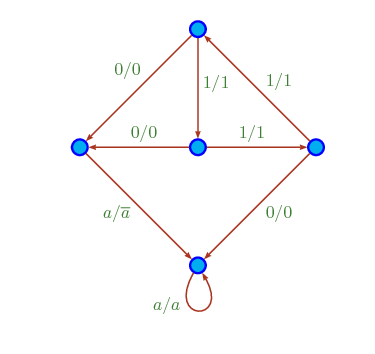
\includegraphics[scale=0.5]{figures/grigorchuk}
\end{center}
\caption{Grigorchuk's 5 state machine}
\end{figure}

\section{Background}
An \defn{automaton} is formally a triple $(Q, \Sigma, \delta)$, where
$Q$ is some finite state set, $\Sigma$ is a finite alphabet of
\defn{symbols}, and $\delta$ is a transformation on $Q \times \Sigma$.
Automata are typically viewed as directed graphs with vertex set $Q$
and an edge labeled $x \mid y$ between $u, v$ if
$(u, x)\delta = (v, y)$.

\begin{center}
\begin{tikzpicture}[
        > = stealth, % arrow head style
        shorten > = 1pt, % don't touch arrow head to node
        auto,
        node distance = 2.5cm, % distance between nodes
        semithick % line style
    ]
    \tikzstyle{every state}=[
        draw = black,
        thick,
        fill = white,
        minimum size = 4mm
    ]
    \node[state] (start) {$u$};
    \node[state] (halt) [right of=start] {$v$};
    \path[->] (start) edge node {$x \mid y$} (halt);
\end{tikzpicture}
\end{center}

One interprets this as if $\A$ is in state $u$ and reads symbol $x$,
then $\A$ transitions to state $v$ and outputs symbol $y$. A
computation within $\A$ may then start at some state $q_0$, and on
input $\alpha_0 \alpha_1 \ldots \alpha_k$, output
$\beta_0 \beta_1 \ldots \beta_k$, where
$(q_i, \beta_i) = (q_{i-1}, \alpha_i)\delta$ for all $i = 0\ldots k$.

As in the above case, where $\delta$ outputs exactly one character for
every transition, we call the automaton $\A$ \defn{alphabetic}. An
automaton is called \defn{invertible} when every state in $Q$ has some
bijection $\pi \in \mathfrak{G}_n$ on $\Sigma$ such that
$(u, x)\delta = (v, \pi(x))$. Here, $\mathfrak{G}_n$ denotes the
symmetric group on $n$ letters. A state in $\A$ is a \defn{copy state}
if $\pi$ is the identity permutation and is a \defn{toggle state}
otherwise. The present paper is concerned only with invertible,
alphabetic automata.

\subsection{Actions on the infinite tree}

We may identify the set $\Sigma^*$ with an infinite, regular tree of
degree $|\Sigma|$. The root is labelled with the empty string
$\epsilon$, and a vertex labelled $w$ has the child $wa$ for each
$a \in \Sigma$. Out of convenience, we will frequently conflate a
vertex with its label.

% TODO make this less ugly
\begin{figure}
\begin{center}
\begin{tikzpicture}[
        > = stealth, % arrow head style
        shorten > = 1pt, % don't touch arrow head to node
        auto,
        node distance = 1.5cm, % distance between nodes
        semithick % line style
    ]
    \tikzstyle{every state}=[
        draw = black,
        thick,
        fill = white,
        minimum size = 3mm
    ]
    \node[state] (root) {$\epsilon$};
    \node[state] (s0) [below left  of=root] {$0$};
    \node[state] (s1) [below right of=root] {$1$};
    \node[state] (s00) [below left  of=s0] {$00$};
    \node[state] (s01) [below right=0.56cm and 0.1cm of s0] {$01$};
    \node[state] (s10) [below left=0.56cm and 0.1cm of s1] {$10$};
    \node[state] (s11) [below right of=s1] {$11$};
    \path[->] (root) edge node {} (s0);
    \path[->] (root) edge node {} (s1);
    \path[->] (s0) edge node {} (s00);
    \path[->] (s0) edge node {} (s01);
    \path[->] (s1) edge node {} (s10);
    \path[->] (s1) edge node {} (s11);
\end{tikzpicture}
\caption{$\textbf{2}^*$ interpreted as the infinite binary tree}
\end{center}
\end{figure}

Each state $q \in Q$ acts on the corresponding tree, sending vertex
$w$ to $wq$. Moreover, if $\alpha \alpha' q = \beta \beta'$, then
$\alpha q = \beta$, for any
$\alpha, \alpha', \beta, \beta' \in \Sigma^*$. Which is to say, $q$'s
action on the tree is an adjacency-preserving map and is thus an
endomorphism on the tree. Additionally, $q$ is length-preserving, and
thus preserves levels of the tree (and thus is an automorphism of the
tree).

% TODO to talk about faithful actions, need some wreath recursion
% background. Maybe move this generalization after the wreath
% recursion part?
We extend the action of $Q$ on $\Sigma^*$ to words $q = q_1\ldots q_n$
over $Q^+$ by \[ wq = (\ldots((w q_1) q_2)\ldots q_n). \]

This computation corresponds with running $\A$ starting at state $q_1$,
then taking that output and running it through the machine starting at
state $q_2$, and so on. We adopt the convention of applying functions
from the right here. In this way, function composition corresponds
naturally with string concatenation.

Thus, there is a natural homomorphism
$\phi : Q^+ \rightarrow \operatorname{Aut}\textbf{2}^*$, where
$\operatorname{Aut}\textbf{2}^*$ denotes the semigroup of automorphisms of the
tree $\textbf{2}^*$. We denote the image of $\phi$ by $\Sigma(\A)$.

\subsection*{Semigroup theory}

A \defn{semigroup} is a set $S$ paired with a binary operation
$f : S \times S \rightarrow S$ such that $S$ is closed under $f$ and
$f$ is associative over $S$. Any set of endofunctions forms a
semigroup under composition.

A semigroup is called \defn{Abelian} when its corresponding binary
operation is commutative.

For an automaton $\A$, we denote by $S(\A)$ the semigroup generated by
$Q$ under composition. $\A$ is said to be \defn{commutative} or
\defn{Abelian} when $S(\A)$ is Abelian. We write $G(\A)$ for the group
generated by the elements of $Q$ and their inverses.

One may also speak about $S(\A)$ and $G(\A)$ without explicit reference
to an automaton $\A$, yielding the corresponding definition:
\begin{definition}
  We call a semigroup $S$ an \emph{automaton semigroup} if there is
  some automaton $\A$ with $S \simeq \Sigma(\A)$. Similarly, a group
  $G$ is called an \emph{automaton group} if $G \simeq \Sigma(\A)$ for
  some automaton $\A$.
\end{definition}

\subsection*{Wreath Recursions}
Any automorphism $f$ of $\Sigma^*$ can be written in the recursive form:
\[ f = (f_{\alpha_1}, f_{\alpha_2}, \ldots, f_{\alpha_n})\tau \] where
$n = |\Sigma|$ and each $f_\alpha$ is an automorphism of a subtree of
the root. Here, $\tau$ is some permutation on $\Sigma$. In the case
where $\Sigma = \{0, 1\}$, we have $f = (f_0, f_1)\sigma$ where
$\sigma$ denotes transposition. If $f = (f_0, f_1)\sigma$, $f$ is said
to be \defn{odd}. If $f = (f_0, f_1)$, f is said to be
\defn{even}. That is to say, automorphisms may be classified as even
or odd depending on their action on the first level of the tree.

The set of even automorphisms form a subgroup $H$ of index 2 in
$G(\A)$.

% TODO these next two paragraphs are fishy
The automorphism semigroup of $\Sigma^*$ decomposes into a recursive
wreath product
\[
  \operatorname{Aut}\Sigma^* = \operatorname{Aut}\Sigma^* \wr
  \tau_\Sigma
\]
where $\tau_\Sigma$ is the tranformation semigroup on $\Sigma$. Which
is to say,
\[
  \operatorname{Aut}\Sigma^* =
  \underbrace{(\operatorname{Aut}\Sigma^* \times \ldots \times
    \operatorname{Aut}\Sigma^* )}_\text{$n$ times} \rtimes
  \tau_\Sigma.
\]

\begin{definition}
  Define \emph{residuation maps}
  $\partial_a : S(\A) \rightarrow S(\A)$ that map
  $f = (f_0, f_1)\sigma$ to $f_a$, and a \emph{parity map}
  $\textsf{par}$ such that $\textsf{par}(f) = \sigma$.
\end{definition}

When restricted to the subgroup $H$ of even automorphisms.
residuation maps are group homomorphisms

Note that a subgroup $G$ of $\operatorname{Aut}(2^*)$ need not be
closed under residuation; if it is, we call it \emph{self-similar} or
\emph{state-closed}. In this case, the wreath characterization in the
full automorphism group carriers over and we have
$G \cong (G \times G) \rtimes \tau_{\textbf{2}}$.

% TODO stress that this is a group homomorphism on H

% TODO running example
% TODO an example here would be very very useful

% TODO
% Cosets thing

\begin{example}
  The following automaton is called $A^3_2$, a notable member of the
  class of \emph{cycle-cum-chord} automata discussed in
  \cite{sutner:iterating}.
  % \vspace{-5em}
  \begin{center}
  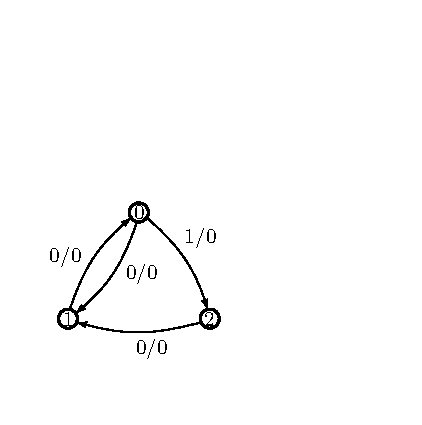
\includegraphics[scale=0.4]{figures/a32-extended}
  % \vspace{-1em}
  \end{center}
  Write $\underline{i}$ for the automorphism corresponding to state
  $i$. Then we have the following wreath recursions:
  $\underline{0} = (\underline{1}, \underline{2})\sigma$,
  $\underline{1} = (\underline{0}, \underline{0})$,
  $\underline{2} = (\underline{1}, \underline{1})$. Correspondingly,
  we can see $\partial_0 \underline{0} = \underline{1}$ and
  $\partial_1 \underline{0} = \underline{2}$.
\end{example}

\section{Decision Problems}

Automaton semigroups exhibit many interesting and nuanced
computability properties. While it is an easy result that the
\decprob{word problem} is solvable in such semigroups, similar
group-theoretic problems such as the \decprob{conjugacy problem} and
\decprob{finiteness problem} have been shown to be undecidable
(see \cite{sunic:conj}, and \cite{gillibert:finite}, respectively).

Various other semigroup theoretic decision problems have recently been
considered for small classes of semigroups by Cain in
\cite{Cain09:dec_prob}. We consider a subset of his distinguished
properties in the automaton semigroup case here.

% TODO finitely generated and other background

\subsection{\decprob{IsAbelian} is polynomial time}

We present a polynomial time algorithm to determine if an input
automaton $\A$ is Abelian.

For a binary invertible automaton $\A$, define the \emph{gap} of an
automorphism $f \in G(\A)$ to be
$\gamma_f = (\partial_0 f)(\partial_1 f)^{-1}$.

The following result is adapted from \cite{okano:thesis}.

\begin{lemma}
  $\A$ is Abelian if and only if all even automorphisms in $S(\A)$
  have gap $I$ and odd automorphisms share the same constant gap.
\end{lemma}

\begin{proof}
Suppose $\A$ is Abelian; so $fg = gf$ for all $f$, $g$ in $S(\A)$.
If $f$ and $g$ are both odd, residuating both sides gives
\[
  (\partial_a f)(\partial_{\overline{a}}g) =
  \partial_a (fg) =
  (\partial_a gf) =
  (\partial_a g)(\partial_{\overline{a}}f)
\]
which yields $\gamma_f = \gamma_g$. Here, $\overline{a}$ denotes $1 - a$.
If $f$ is even and $g$ odd, without loss of generality, we have
\[
  (\partial_0f)(\partial_0 g) = 
  \partial_0(fg) =
  \partial_0(gf) =
  (\partial_0g)(\partial_1 f)
\]
which, with algebraic manipulation, yields $\gamma_f = I$.

Conversely, first suppose $f$ and $g$ are both odd. Then
$fg = (\partial_0 f \partial_1 g, \partial_1 f \partial_0 g)$ and
$gf = (\partial_0 g \partial_1 f, \partial_1 g \partial_0 f)$. Since
$\gamma_f = \gamma_g$, these wreath recursions are the same. If $f$ is
even and $g$ odd,
$fg = (\partial_0f \partial_0g, \partial_1 f \partial_1 g)\sigma$ and
$gf = (\partial_0g \partial_1f, \partial_1 g \partial_r f)\sigma$,
which are the same expansion, since $\gamma_f = \gamma_g$.

If $f$ and $g$ are both even, both directions of the claim follow by
induction.
\end{proof}

\begin{definition}
  For an automaton $\A$ with states $s_1 \ldots s_n$, the
  \emph{inverse automaton} of $\A$, denoted $\A^{-1}$, has state set
  $t_1, \ldots t_n$ and transitions
  $\partial_a t_i = \partial_{\overline{a}} s_i$, with $t_i$ a toggle state
  if and only if $s_i$ is as well.
\end{definition}

It is easy to verify by induction that $t_i = s_i^{-1}$ for all $i$.

\begin{definition}
  For an automaton $\A = (Q,\Sigma, \delta)$, the \emph{acceptor of
    $\A$ at $t$}, denoted $\A(t)$, is a partial DFA with state set
  $Q$, input alphabet $\Sigma \times \Sigma$, and transitions
  $s \stackrel{a \times b}{\longrightarrow} s'$ for each transition
  $t \stackrel{a \mid b}{\longrightarrow} t'$ in $\A$. Every state is
  accepting. The first track of the alphabet $\Sigma\times\Sigma$ may
  be interpreted as the input to $\A$, and the second, the output of
  $\A$.
\end{definition}

\begin{lemma}
  % $\A(t)$ accepts all convoluted pairs of 
  The language of the acceptor $\A(t)$ is
  \[
    \{(x_1, y_1)(x_2, y_2),\ldots,(x_n, y_n) \mid y_1\ldots y_n =
    (x_1,\ldots x_n)t \}
  \]
\end{lemma}
\begin{proof}
  By induction on the length of the input string.
\end{proof}

\begin{definition}
  For an automaton $\A = (Q, \Sigma, \delta)$, the \emph{product
    automaton} $\A \times \A$ is a machine with state set $Q\times Q$
  and transition function defined by
  $\partial_a (s_1, s_2) = (\partial_a s_1, \partial_{a s_1} s_2)$.
\end{definition}

We can see by induction that the behavior of each state $(s_1, s_2)$
in the product automaton corresponds to the word $s_1 s_2 \in S(\A)$.

% TODO get a precise bound. TODO use fancy Union-Find data structure
% for equivalence checking
\begin{theorem}
  There is a polynomial time algorithm to check if an automaton $\A$
  is Abelian.
\end{theorem}

\begin{proof}
  On input automaton $\A$, build the inverse automaton
  $\A^{-1}$. Construct the product automaton $\A\times \A^{-1}$. Then
  for each toggle state $t_i$ of $\A$, for the state
  $s_i = (\partial_1 t_i, \partial_1 t_i^{-1})$ in $\A\times \A^{-1}$,
  construct the acceptor DFA $(\A\times \A^{-1})(s_i)$. Verify all the
  constructed DFAs are equivalent.
\end{proof}

The reader may be interested to note that this product automaton
construction also provides proof that the word problem for automaton
semigroups is decidable.

\subsection{Automorphism \decprob{Membership}}

This section considers the subsemigroup $S(\A)$ of
$\operatorname{Aut}\textbf{2}^*$ generated by the associated automophisms of
an invertible binary transducer. We assume minimality throughout this
section.

We provide proof that the automorphism membership question is
decidable in the Abelian case, and discuss partial work toward the
general case. Some necessary background from
\cite{NekrashevychSidki04:automorphisms} is outlined below.

\subsubsection{Linear algebraic background}

% TODO this is so poorly worded
\begin{theorem}
  If $\A$ is Abelian, then $G(\A)$ is isomorphic to either a finite
  Boolean group or to $\Z^m$ for some $m \geq 1$. In the latter case,
  there is an isomorphism $\phi : G(\A) \rightarrow \Z^m$ satisfying
  the following recursion
\[
  \phi^{-1}(v) =
  \begin{cases}
    (\phi^{-1}(A\cdot v), \phi^{-1}(A \cdot v)) & \text{if $\phi^{-1}$ is even}\\
    (\phi^{-1}(A\cdot v - r), \phi^{-1}(A \cdot v + r)) &
    \text{otherwise}
  \end{cases}
\]
where $A \in GL(m,\Q)$ and $v \in \Q^m$. Additionally, for all
$v \in \Z^m$, $A\cdot v \in \Z^m$ or $A\cdot v \pm r \in \Z^m$.
\end{theorem}

We call the matrix $A$ above the \defn{residual matrix} of $A$. The
vector $r$ is referred to as the \defn{residual vector}. Put
differently, this theorem specifies that when $\A$ is Abelian,
residuation is an affine map.

We have the following properties of the residual matrix $A$:

% TODO don't conflate the automaton A with the matrix A
\begin{theorem}
If $G(\A) \cong \Z^m$ and $A$ is its associated
residual matrix, $A$ satisfies the following properties:
\begin{enumerate}
\item $A$ is contracting; its spectral radius is less than 1
\item $A$ is 1/2-integral, meaning that $A^{-1}$ is a subgroup of
  index 2 in $\Z^m$. Therefore $A$ be represented as
  \[
    \begin{bmatrix}
      \frac{a_{1,1}}{2} & a_{1,2} & \cdots & a_{1,m} \\
      \frac{a_{2,1}}{2} & a_{2,2} & \cdots & a_{2,m} \\
      \vdots & \vdots & \ddots & \vdots \\
      \frac{a_{m,1}}{2} & a_{m,2} & \cdots & a_{m,m}
    \end{bmatrix}
  \]
  where all
  $a_{i,j}$ are integers.
\item The characteristic polynomial $\chi_A(x)$ is irreducible over
  $\Q$ and has the form
  \[ \chi_A(x) = x^m + \frac{1}{2}g(x) \] for some $g \in \Z[x]$ of
  degree at most $m-1$. In particular, the constant term is
  $+-\frac{1}{2}$.
\item $A$ is invertible and the characteristic polynomial
  $\chi_{A^{-1}}(x)$ is integral and irreducible over $\Q$. From
  property 2, Laplace expansion yields that $A^{-1}$ is an integral
  matrix that is similar to the companion matrix of $\chi_{A^{-1}}(x)$
  over $\Q$.
\end{enumerate}
\end{theorem}

The Latimer and MacDuffee proved the following theorem in
\cite{latimer:corresp}:

\begin{theorem}
  If $p(x) \in \Z[x]$ is monic and irreducible, the $GL(m, \Z)$
  similarity classes of integral matrices whose characteristic
  polynomial coincides with $p(x)$ is in one-to-one correspondance
  with ideal classes of the ring $\Z[\theta]$, where $\theta$ is any
  root of $p(x)$.
\end{theorem}

Property 1 of theorem 3 provides a bound on the coefficients of
$\chi_A(x)$. When combined with property 4 and the above theorem, it
can be shown that, for fixed $m$, there exist only finitely many
possibilities of $A$, up to $GL(m, \Z)$ similarity.

% Interesting typesetting decision here: one parenthesis is
% italicized, while its match is not
\begin{definition}
  Take $G$ to be some self-similar group. We may construct the
  \emph{complete group automaton} (occasionally abbreviated as the
  \emph{complete automaton)} for $G$, written $\mathcal{C}_G$, as
  follows: the automaton has $G$'s carrier set as state set with
  transitions $f \stackrel{a\mid af}{\longrightarrow} \partial_a f$.
\end{definition}

Of course in general,
this invertible automaton will be infinite, but certainly
$\mathcal{S}(\mathcal{C}_G)$ is a group and ismorphic to $G$. The more
interesting case is when $G$ may be represented in terms of a finite
automaton. Toward this end, call $G$ \emph{finite-state} if for all
$f \in G$, the number of residuals $\partial_w f$ is finite. If $G$ is
self-similar, finite-state, and finitely generated, we can construct
the \emph{group automaton} $\mathcal{A}_G$, a binary Mealy automaton,
just like the complete group automaton, but with state set restricted
to the collection of all residuals of the generators of $G$. Of
course, the group generated by $\mathcal{A}_G$ is isormorphic to
$G$. One need to be careful, however; the semigroup may be
different. Pleasantly, $\mathcal{A}_G$ is minimal by construction.

The following lemma is adapted from \cite{okano:thesis}. 

\begin{lemma}
  For any admissible $(A, r)$, the complete automaton $\mathcal{C}$
  over $A$ and $r$ has only finitely many subautomata, each of which
  has finitely many states.
\end{lemma}
\begin{proof}
  Fix some state $v \in \Z^m$. Since residuation is an affine map, we
  may write every descendent $w$ of $v$ as a monic polynomial over $A$:
  \[
    w = A^nv + \sum_{i = 0}^{n-1}d_i A^i r
  \]
  where $d \in \{-1, 0, 1\}$. This comes down to using a redundant
  numeration system similar to base 2, but with a symmetric digit set.
  Letting $\norm{\cdot}$ denote both the norm over $\Q^m$ and the
  induced matrix norm, we have the bound
  \[
    \norm{w} \leq \norm{A^n}\norm{v} + \norm{r} \sum_{i=0}^{n-1} \norm{A^i}
  \]
  by the triangle inequality. Taking the limit as
  $n\rightarrow\infty$, $\norm{A^n}$ goes to 0, as
  $\norm{A^n} = \lambda^n$, where $\lambda$ is the spectral radius of
  $A$ (and $\lambda < 1$ by Theorem 3). Thus, in the limit, we have a
  bound on $\norm{w}$ that is independent of $\norm{v}$.

  Put differently, this says that, eventually, all descendents of $v$
  are bounded from above by some expression independent of $v$. Since
  any ball of finite radius around 0 in $\Z^m$ is finite, this implies
  that there must be finitely many strongly connected components in
  $\mathcal{C}$, each of finite order.
\end{proof}

\begin{lemma}
  One may compute all such subautomata.
\end{lemma}
\begin{proof}
  Brute force search in the finite ball around 0. The radius of the
  ball may be effectively computed from $\lambda$.
\end{proof}

\begin{example}
The following automata represent all subautomata of
the complete automaton generated with residual matrix
\[
  A = \begin{bmatrix}
    -1 &1\\
    -\frac{1}{2} & 0
    \end{bmatrix}
\]
and residual vector $r = [-1, -\frac{3}{2}]^T$.

\vspace{-5em}
\begin{center}
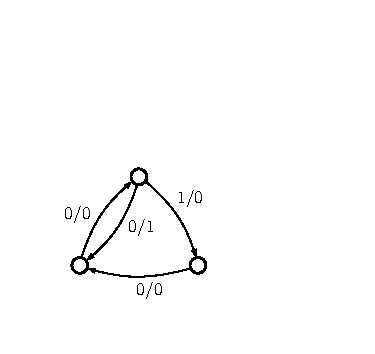
\includegraphics[scale=0.5]{figures/a32}
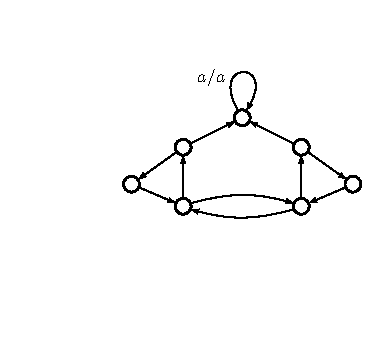
\includegraphics[scale=0.5]{figures/bowtie}
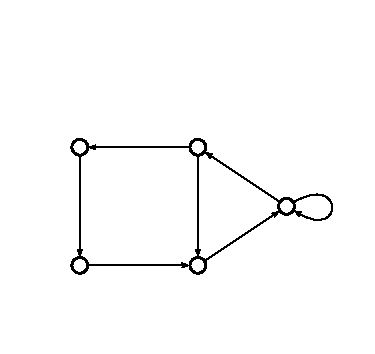
\includegraphics[scale=0.5]{figures/pent}
\end{center}
The top state of $A^3_2$ (seen earlier in example 1) corresponds with
$e_1 \in \Z^2$. One can check that $A(Ae_1 - r) = e_1$, corresponding
with going around the shorter loop.
\end{example}

\begin{definition}
  For a residual matrix $A$ and residual vector $r = A \cdot e_1$, the
  \emph{principal automaton} is the automaton generated from closure
  of $e_1$ under residuation defined by the pair $(A, r)$.
\end{definition}

\subsubsection{\decprob{Membership} is decidable in the Abelian case}

\begin{definition}
  The automorphism \decprob{Membership} problem takes as input two
  automata, $\A$ and $\B$, a distinguished automorphism $f \in \A$
  corresponding to some state $p$, and $\B$'s residual matrix and
  vector $A$ and $r$, and ouputs whether $f \in S(\B)$.
\end{definition}

State-closed, finite-state automorphisms admit the natural
computational representation as automata. It is worth noting that our
\decprob{Membership} problem differs from the \decprob{Word Problem}:
the word problem considers candidates given as words over the
generators of a semigroup $S$; here our candidates are raw
automorphisms.

Returning to \decprob{Membership}, one thus needs to check if there is
some product automaton
\[
  \mathcal{D} = \B_{p_1} \times \B_{p_2} \times \ldots \times \B_{p_n}
\]
that implements $f$. We have no computable bound on $n$, so a priori
this only semidecidable (this is a running theme).
% TODO maybe mention this open problem

\begin{theorem}
  Automorphism \decprob{Membership} in $S(\B)$ for a principal Abelian
  automaton $\B$ is decidable.
\end{theorem}
\begin{proof}
  Given as input an automaton $\A$ and a principal Abelian automaton
  $\B$, we determine if $f = \A(p)$ is in the semigroup generated by
  $\B$.

  % TODO justify - adversay and Knuth Normal Form
  It suffices to simply check if $f$ is equivalent to any automorphism
  in any of the subautomata of $\mathcal{C}_\B$.

  Consider the complete automaton $\mathcal{C}$ for $\B$. Define $g$
  to be the automorphism defined by $\mathcal{D}$. After minimization,
  $\mathcal{D}$ produces a subautomaton of $\mathcal{C}$ that consists
  of a ``transient part'' and a copy of $\B$ (there may be strongly
  connected components in the transient part, but they are not
  subautomata). Hence, there is some word $w$ such that $\partial_w g$
  is just a single state in the copy of $\B$.

  % Since a simulation $g$ of $f$ must hold for all inputs, it suffices
  % to check that 

  % In fact, for all $u$, there is a $w$ such that $\partial_{ww}g$ is
  % atomic. Essentially this just means that $g$ is strongly tame.

  % TODO do all of the subautomta span??
  % If 
\end{proof}

{\color{TODO}
% We may safely assume that $\A$ is minimal. Then is looks like $\A$ has
% to have $\B$ as a subautomaton to satisfy this ultimate atomicity
% condition, plus a transient part sitting on of $\B$. It should be
% decidable if things match up.

% If $\B$ is not principal, there are multiple subautomata of $C$ to
% content with, but that should not make a major difference. Ditto if
% $\B$ is just a random subautomaton of $C$.

% TODO
% If same A and r, just identity check.
% If same A, rdifferent r - nontrivial now.
%   - Just a linear subspace problem.
%   - We can assume we have the info up front
%   - Answer is no qne-way and yes the other (bowtie and A32)
% Different A:
%   - Charpoly changes here. Tell you about the identities.
%   - TODO
%   - just write out the equations for the thing you're testing
%
% TODO - come up with two automata with separate A, r, A', r'
%        but there's a function in one machine that can be simulated in the
%        other.
}

\subsubsection{\decprob{Membership} is open in the general case}

The decidablity of \decprob{membership} is arguably the most important
open problem relevant to this thesis. Its decidablity would imply the
decidability of \decprob{IsGroup}, as one could simply check that the
inverse of each generator is contained in $\mathcal{S}(\A)$.

\subsection{\decprob{IsGroup}}
\begin{definition}
  The \decprob{IsGroup} decision problem takes as input an automaton
  $\A$ and answers the question ``is $S(\A) = G(\A)$?''
\end{definition}

\begin{example}
  There exist automata for which $S(\A)$ is not a group; the adding
  machine in figure 3 is such a machine. Viewing the input string as a
  natural number in reverse binary, one can see that it adds one to
  the input.
\end{example}
\begin{figure}
\begin{center}
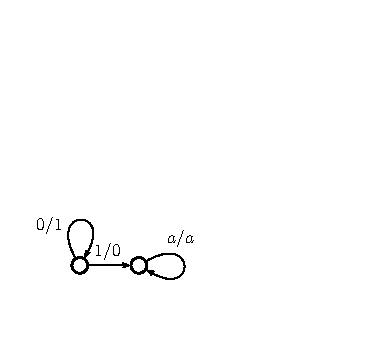
\includegraphics[scale=0.7]{figures/adder}
\end{center}
\caption{The adding machine}
\end{figure}

\begin{proposition}
  \decprob{IsGroup} is decidable in the Abelian case.
\end{proposition}

This follows immediately from a decidable automorphism
\decprob{Membership} problem: simply check for membership of the
identity function and the inverse of each generator.

Despite a fair amount of effort, \decprob{IsGroup} is still open in
the general case. Our work on \decprob{Knapsack} and
\decprob{Membership} represent much partial work toward a solution.

\subsection{\decprob{Knapsack} is undecidable for automaton semigroups}
We follow a proof strategy inspired by \cite{Konig15:knapsack}.

% TODO need to use sets of variables for full formality

\subsubsection{Exponential Equations}

Suppose $\mathcal{X}$ is a countably infinite set of variables.
\begin{definition}
  An \emph{exponential equation} $E$ over a semigroup $S$ is an equation of 
  formal products of the form
  \[
    s_1^{x_1} s_2^{x_2}\cdots s_l^{x_l}
    = t_1^{y_1} t_2^{y_2}\cdots t_l^{y_l}
  \]
  where each $x_i, y_i$ is in $\mathcal{X}$ and each $s_i, t_i$ is in $S$. Note
  that we do not require the $x_i$'s and $y_i$'s to be distinct.
\end{definition}

Denote by $\operatorname{Var}(E)$ the set of all variables appearing
in $E$.
\begin{definition}
  For a finite set $X$ and semigroup element $s$, the set of
  \emph{$X$-solutions} of the equation $E$ is the collection of maps
  \[
    S_X(E = s) = \{ v : X \rightarrow \N \mid
    s_1^{v(x_1)} s_2^{v(x_2)}\cdots s_l^{v(x_l)} = s
    \text{ \normalfont in } S
    \}
  \]
\end{definition}

The upcoming reduction involves taking direct products of semigroups,
and so we will need the following strategy to transform exponential
expressions over a semigroup $S$ to equivalent exponential expressions
over a direct product containing $S$.

% TODO define base element
To this end, suppose we have exponential expressions $E_i$ for
$i = 1\ldots n$, each with corresponding semigroups $S_i$. In each
$E_i$, replace the base element $s_i$ with the element
\[
  (\underbrace{1, \ldots, 1}_\text{$i-1$}, s_i,
   \underbrace{1, \ldots 1}_\text{$n-i$}) \in \prod_i S_i.
\]
Then take the formal product of each new $E_i$.

\subsubsection{Undecidability of \decprob{Knapsack}}

% TODO phrase in terms of variables
\begin{definition}
  We define the \decprob{Knapsack Problem} as follows: given as input
  generators $g_1 \ldots g_k$ and a target semigroup element $g$, do
  there exist natural numbers $a_1\ldots a_k$ such that
  \[ g_1^{a_1} \cdots g_k^{a_K} = g \]
\end{definition}

% The reader may be more familiar with the Knapsack variant from
% complexity theory, that asks if
This decision problem is named as such due to its similarity with the
\emph{unbounded knapsack problem}, which asks, for items indexed from
$i = 1$ to $n$, each with value $v_i$ and weight $w_i$, to maximize
the sum
\[
  \sum_{i=0}^n v_i x_i
\]
where $x_i$ denotes the number of times item $i$ is
used. Additionally, it is required that $\sum_{i=0}^nw_ix_i \leq W$
for some weight $W$, with each $x_i \geq 0$.

In our variant, the indexed items are group elements, each with weight
$g_i$, and repetition $a_i$. Rather than seeking to maximize the
formal product, the variant asks to hit a target value.

% TODO phrase in terms of variables
\begin{definition}
  The \decprob{Generalized Knapsack Problem} has as input generators
  $g_1 \ldots g_k, h_1, \ldots h_l$, and has as output whether there
  exist natural numbers $a_1\ldots a_k, b_1, \ldots, b_l$ such that
  \[ g_1^{a_1} \cdots g_k^{a_k} = h_1^{b_1} \cdots h_l^{b_l} \]
\end{definition}

% TODO reducing "to"?
We demonstrate that the \decprob{Generalized Knapsack Problem} is
undecidable in the class of automaton semigroups by reducing from
Hilbert's tenth problem. The undecidablity of the \decprob{Knapsack
 Problem} easily follows.

\begin{definition}
  We define the decision problem \decprob{Hilbert} as following:
  ``given a polynomial $P(x_1, \ldots, x_n) \in \Z[x_1, \ldots, x_n]$
  and an integer $a$, do there exist values $y_i \in \N$ such that
  $P(y_1, \ldots, y_n) = a$?''
\end{definition}

It is well-known that there exist polynomials for which
\decprob{Hilbert} is undecidable, see \cite{Matiyasevich:hilbert} for
details.

One can show that the Heisenberg semigroup
\[
  H_3(\mathbb{N}) = \left\{
      \begin{bmatrix}
        1 & a & c \\
        0 & 1 & b \\
        0 & 0 & 1
      \end{bmatrix}; a, b, c \in \mathbb{N}
    \right\}
\]
is an automaton semigroup \cite{Bondarenko:heisenberg}. Moreover, the
class of automaton semigroups is closed under direct products, proven
by Cain in \cite{Cain09:auto_sg}. We denote elements of $H_3(\N)$ as
\[
  H_{x,y,z} = 
      \begin{bmatrix}
        1 & x & z \\
        0 & 1 & y \\
        0 & 0 & 1
      \end{bmatrix}
\]

\begin{proposition}
  There exist fixed constants $d,e \in \N$ and an exponential
  equation $E$ of the form
  \[ s_1^{x_1} s_2^{x_2}\cdots s_n^{x_n} = t_1^{y_1} t_2^{y_2}\cdots
    t_n^{y_n} \] with $s_i, t_i \in G = H_3(\N)^d \times \Z^e$ for which the
  \decprob{Generalized Knapsack} problem is undecidable.
\end{proposition}

% TODO consider inserting actual automata diagrams for the G_i's.
\begin{proof}
  From the input polynomial, $P(x_1, \ldots, x_n)$ and target value
  $a$, we separate the positive and negative terms of $P$ to obtain an
  equation of the form
  \[
    P_+(x_1, \ldots, x_n) = P_-(x_1, \ldots, x_n, a)
  \]
  where every coefficient in $P_+$ and $P_-$ is positive. From this
  equation, we construct a system $S$ of equations, where each
  equation has one of the following forms: $x\cdot y = z$,
  $x+y = z$, $x = c$ (for $c \in \Z$).  We will have that the equation
  $P(x_1,\ldots, x_n) = a$ has a solution in $\N$ if and only if the
  system of equations $S_a = S \cup \{x_0 = a\}$ has a solution in
  $\N$. Let $X$ be the set of variables that occur in $S_a$.

  Take a natural number $a$ (the input of the reduction). Assume that
  $S_a$ contains $d$ equations of the form $x\cdot y$, and $e$ many
  equations of the form $x+y = z$ or $x = c$. We enumerate these
  equations as $E_1, \ldots E_{d+e}$, where the first $d$ equations
  are of the form $x\cdot y = z$. Then set $G_i = H_3(\N)$ for each
  $i \leq d$ and set $G_i = \N$ for each $i > d$. For every $i$, we
  define an element $g_i$ and an exponential expression $E_i$ over
  $G_i$ as follows:

  % TODO need to reformat all of this into two-sided equations
  \textit{Case 1:} $E_i = (x \cdot y = z)$. Thus we have
  $G_i = H_3(\N)$. Set $g_i$ to be the identity matrix in $H_3(\N)$
  and consider the following equation:
  \[
    H^x_{1,0,0} =
    \begin{bmatrix}
      1 & x & xy \\
      0 & 1 & y \\
      0 & 0 & 1
    \end{bmatrix} = 
    \begin{bmatrix}
      1 & x & z \\
      0 & 1 & y \\
      0 & 0 & 1
    \end{bmatrix} = 
    H^z_{1,0,0} H^y_{0,0,1} H^x_{1,0,0}
  \]

  A mapping $v : X \rightarrow \N$ is a solution if and only if
  $v(x)v(y) = v(z)$.

  \textit{Case 2:} $E_i = (x+y=z)$ and so $G_i= \Z$. Set $g_i = 0$ and
  consider the equation (written additively in the group $\Z$)
  \[
    x+y-z = 0
  \]
  Then a mapping $v : X \rightarrow \Z$ is a solution if
  and only $v(x) + v(y) = v(z)$.

  \textit{Case 3:} $E_i = (x = c)$. (This includes our distinguished
  equation $x_0 = a$). We have $G_i = \Z$. Then set $g_i = c$ and
  $E_i = x$. Then as usual, a mapping $v$ is a solution if and only if
  $v(x) = c$.

  Finally, define $E$ to be the direct product of the $E_i$'s
  $\prod_{i=1}^d E_i$ and define $g = (g_1, \ldots g_{d+e})$. Then a
  mapping $v$ is a solution to the equation $E = g$ if and only if $v$
  is a solution to the system of equations $S$.
\end{proof} % proposition

\begin{theorem}
  \decprob{Generalized Knapsack} is undecidable in the class of
  automaton semigroups.
\end{theorem}
\begin{proof}

For all $d, e \in \N$, $H_3(\N)^d \times \Z^e$ is an automaton
semigroup. It follows that \decprob{Generalized Knapsack} is
undecidable for automaton semigroups.

\end{proof} % knapsack theorem 

\subsection{A monoid with decidable \decprob{Word Problem} and undecidable \decprob{IsGroup}} 

% TODO monoid definition
We establish the existence of a monoid with decidable
$\decprob{Word Problem}$, but undecidable $\decprob{IsGroup}$. One may
take this result as an intermediate step toward the decidability of
the $\decprob{IsGroup}$ problem for automaton semigroups.

\subsubsection*{Preliminaries}
Here we take a \defn{Turing machine} to be a 6-tuple,
$(Q, \Sigma, \Gamma, \delta, q_0, q_{accept}, q_{reject})$, where $Q$,
$\Sigma$, $\Gamma$ are all finite sets.
$\delta : Q \times \Sigma \rightarrow Q\times \Gamma \times \{L,S,R\}$
is the transition function, $Q$ is the state set, $\Sigma$ is the
input alphabet, $\Gamma \supseteq \Sigma$ is the tape alphabet, $b$ is
some blank symbol, with $b \in \Gamma - \Sigma$, $q_{accept}$ is the
unique accepting final state, and $q_{reject}$ the single rejecting
final state.

We further define a Turing machine \defn{configuration} to be a triple
$(u, q, v) \in \Gamma^* \times Q \times \Gamma^*$. Here, $u$ denotes
the tape contents to the left of the tapehead, $q$ is the current
state, and $v$ begins at the tapehead and extends to the right.

A configuation $C$ for a TM $M$ is said to \defn{yield} configuration
$C'$ if $M$ can step directly from $C$ to $C'$.

For a Turing machine $M$, take $C_M$ to be the set of all valid
configurations of $M$. Then define $CG_M$ to be the graph $(C_M, E)$,
where $(u,v) \in E$ if and only if $u$ yields $v$ in $M$.
\begin{definition}
Define the \emph{canonical computation of $M$ on $w$}.
\[
  \textsf{canon}(M, w) : \mathcal{T} \times \Sigma^*
      \rightarrow
       C_M^*\cup C_M^\omega
\]
to be the function that maps input $w$ to the sequence of
configurations $M$ takes on while computing over $w$. Note that
$\textsf{canon}(M, w)$ will be a finite sequence if and only if $M$
halts on $w$.
\end{definition}

Certainly, not every configuration in $C_M$ will be along the sequence
$\textsf{canon}(M,w)$. Which is to say, there are unreachable
configurations.

Informally, a \defn{self-verifying Turing machine} $S$ is one that, at
every step, verifies that the current configuration lies upon the
canonical computation. If $S$ finds that this is not the case, $S$
immediately rejects. Otherwise, the computation steps forward a single
step.

In the configuration graph $CG_S$, there is a path extending from each
valid starting configuration $(\epsilon, q_0, w)$ for
$w \in \Sigma^*$. The remaining states form a countably infinite star
graph with $q_{reject}$ as the center.

\begin{proposition}
  There is a computable\footnote{The reader may interested to find
    that \textsf{sv} is in fact primitive recursive.} function
  $\textsf{sv}$ that maps Turing machines to equivalent self-verifying
  Turing machines.
\end{proposition}

Speaking informally, the new Turing machine $S$ maintains on its tape
a time step $t$, the original input $w$ to our original Turing machine
$M$, and $M$'s current configuration $C$. After simulating each step
of $M$, $S$ will re-run $M$ on $w$ for the first $t$ steps. If this
computation results in $M$ sitting in configuration $C$, $S$
increments $t$, replaces $C$ with the new configuration $C'$, and
proceeds to the next step of $M$. Otherwise, $S$ immediately rejects.

One can show that any invalid configuration will be caught after
finitely many steps, as $S$ manually verifies each and every
configuration. For further reading, see \cite{davis:note_utm},
\cite{davis:defn_utm}, and \cite{shepherdson:machine_config}.

\subsubsection*{The submonoid in question}
Define the Turing machine $M = (Q, \Sigma, \Gamma, \delta, q_0, F)$ to
operate only on the blank tape; for all $s \in \Sigma$,
$\delta(q, s) = (q_{reject}, b, S)$

% TODO need to make the Turing machine maintain a counter, right?

Then take the ambient Abelian group $G_M = (C_M, \cdot)$ whose carrier
set is all configurations of $M$. For $c$, $c'$ in $G_M$, we have
$c = c'$ if and only if $c$ yields $c'$.

\begin{proposition}
  $G_{\textsf{sv}(M)}$ has a decidable word problem.
\end{proposition}

\begin{proof}
  For every word $w$ in $G_{\textsf{sv}(M)}$, there exist nonnegative
  integers $a$, $r$ such that $w = q_{accept}^a
  q_{reject}^r$. Further, we may compute $a$ and $b$. Recall that
  $\textsf{sv}(M)$ maintains a program counter $p$ to the left of the
  input. So we may simply run $M$ for the first $p$ steps and then
  check for configuration equality.

  So then given two words $w_1$, $w_2$ in $G_{\textsf{sv}(M)}$, simply
  compute $a_1$, $r_1$, $a_2$, $r_2$. Then $w$ is in
  $G_{\textsf{sv}(M)}$ if and only if $a_1 = a_2$ and $r_1 = r_2$.
\end{proof}

\begin{proposition}
If $s$ is the start configuration of the Turing
machine, it is undecidable whether $\langle s \rangle$ is a group.
\end{proposition}

% TODO formalize
\begin{proof}
  It is well known that the following language is undecidable
  \[
    \decprob{halts} = \{\langle M \rangle \mid \text{TM $M$ halts on
      $\epsilon$} \}
  \]
  and so we reduce from \decprob{halts}. Given as input a TM $M$, we
  use an oracle for $\decprob{IsGroup}$ as follows: first, compute
  $\textsf{sv}(M)$, and then consider $G_{\textsf{sv}(M)}$. Let $s$ be
  the starting configuration for $M$ on $\epsilon$.

  If $M$ halts, then the submonoid generated by $s$ is the trivial
  group. If $M$ hangs, then $\langle s \rangle$ is the free monoid of
  rank one. So then $\langle s \rangle$ is a group if and only if $M$
  halts. Since $\textsf{sv}(M)$ and $M$ are equivalent, we are done.
\end{proof}

% TODO add gap theorem?

\section{Open Questions}

Much partial work has been attempted toward a proof of the solvability
or unsolvability of the \decprob{IsGroup} problem in the general
case. The monoid presented here serves a sort of bound for this
problem; optimistically suggesting that perhaps the class of automaton
semigroups is not so big as to have an undecidable \decprob{IsGroup}.

There is also a rich area of smaller subclasses of automata to
consider. Godin proved the decidablity of \decprob{Knapsack} for the
class of bounded automata in \cite{Godin:knapsack}. It is natural to
then consider the decidability of other decision problems, such as
\decprob{IsGroup}, \decprob{Isomorphism}, and others.

One may also consider decision problems from a group presentation
angle; all automaton semigroups are recursively presented. If we
restrict our considerations to automaton semigroups whose
presentations are regular, or context-free, does this affect the
decidability of various decision problems? One suspects these
questions are probably quite hard.

Additionally, most of the semigroup-theoretic decision properties
listed in \cite{Cain09:dec_prob} remain open in the class of automaton
semigroups. Notably, determining the decidability of Markov properties
would be of great help to future work.

% TODO mention characterization of complete automata? 1SCC conjecture etc

\nocite{*}\addtocontents{toc}{\protect\vspace{\beforebibskip}}
\addcontentsline{toc}{section}{\refname} \bibliographystyle{plain}
\bibliography{thesis}
\end{document}